\documentclass[12pt, a4paper]{article}

\usepackage[T1]{fontenc}
\usepackage[utf8]{inputenc}
\usepackage[english]{babel}
\usepackage{geometry}
\usepackage{booktabs}
\usepackage{hyperref}
\usepackage{parskip}
\usepackage{microtype}
\usepackage{graphicx}
\usepackage{subcaption}

% Le figure (fig1a, fig1b, fig2, fig3a, fig3b, fig4) vanno caricate su Overleaf
% dentro una cartella chiamata "figs". \graphicspath le cerca automaticamente lì.
\graphicspath{{figs/}{./}}

\geometry{margin=2.5cm}

\title{\textbf{Text Mining and Sentiment Analysis}}
\author{Bombardieri, Ottoboni, Zubani}
\date{}

\begin{document}

\maketitle

\section{Introduction}

We looked at sentiment in Amazon reviews for \textit{Atomic Habits} by James Clear. We wanted to see if different ways of figuring out what people thought would match up with the star ratings they left.

We tried five approaches. First, a simple method looking for words in a list (the Bing lexicon), done both with and without removing stopwords. Then, the same lexicon used through UDPipe, in a basic version and an extended one that also pays attention to negators and words that make things stronger or weaker. Lastly, a Naive Bayes classifier that learned from the star ratings themselves. We used star ratings, simplified to two groups (positive if 4 or 5 stars, negative if 3 stars or below), as our measure of what was real.

\section{Data}

Getting the reviews wasn't easy. Since sites like Amazon load content as you scroll, we had to use a tool called RSelenium to actually control a web browser. We logged in, clicked ``show more'' until we had about a hundred reviews visible, and then saved the whole page's code (the HTML). We scraped the title, review text, and star rating using rvest. Reviews from the UK and those from elsewhere use different codes on Amazon, so we grabbed them separately and then put them together. We converted the ``X.0 out of 5 stars'' type of rating into a simple number from one to five.

We only kept reviews written in English, using a tool called cld2. Mixing languages messes up both the word-list method and the classifier we used. We got 95 reviews after filtering. We had a cleaning function for punctuation, adding spaces, and consistent ellipses.

The main thing we were trying to predict, called \texttt{star\_sent}, took the star ratings and split them into two groups: four or five stars meant ``positive,'' and one to three stars meant ``negative.''

\section{Results and Discussion}

\subsection{Exploratory Analysis}

Looking at the reviews, we saw that most of them were really positive, which makes sense for reviews people choose to leave (Figure~\ref{fig:explore}). If you just listed the most common words after getting rid of stopwords, you'd get a basic idea of what people were talking about (Figure~\ref{fig:topwords}): terms like book, habits, read and life show the reviews really centre on the reading experience.

\begin{figure}[h]
\centering
\begin{subfigure}{0.45\textwidth}
\centering
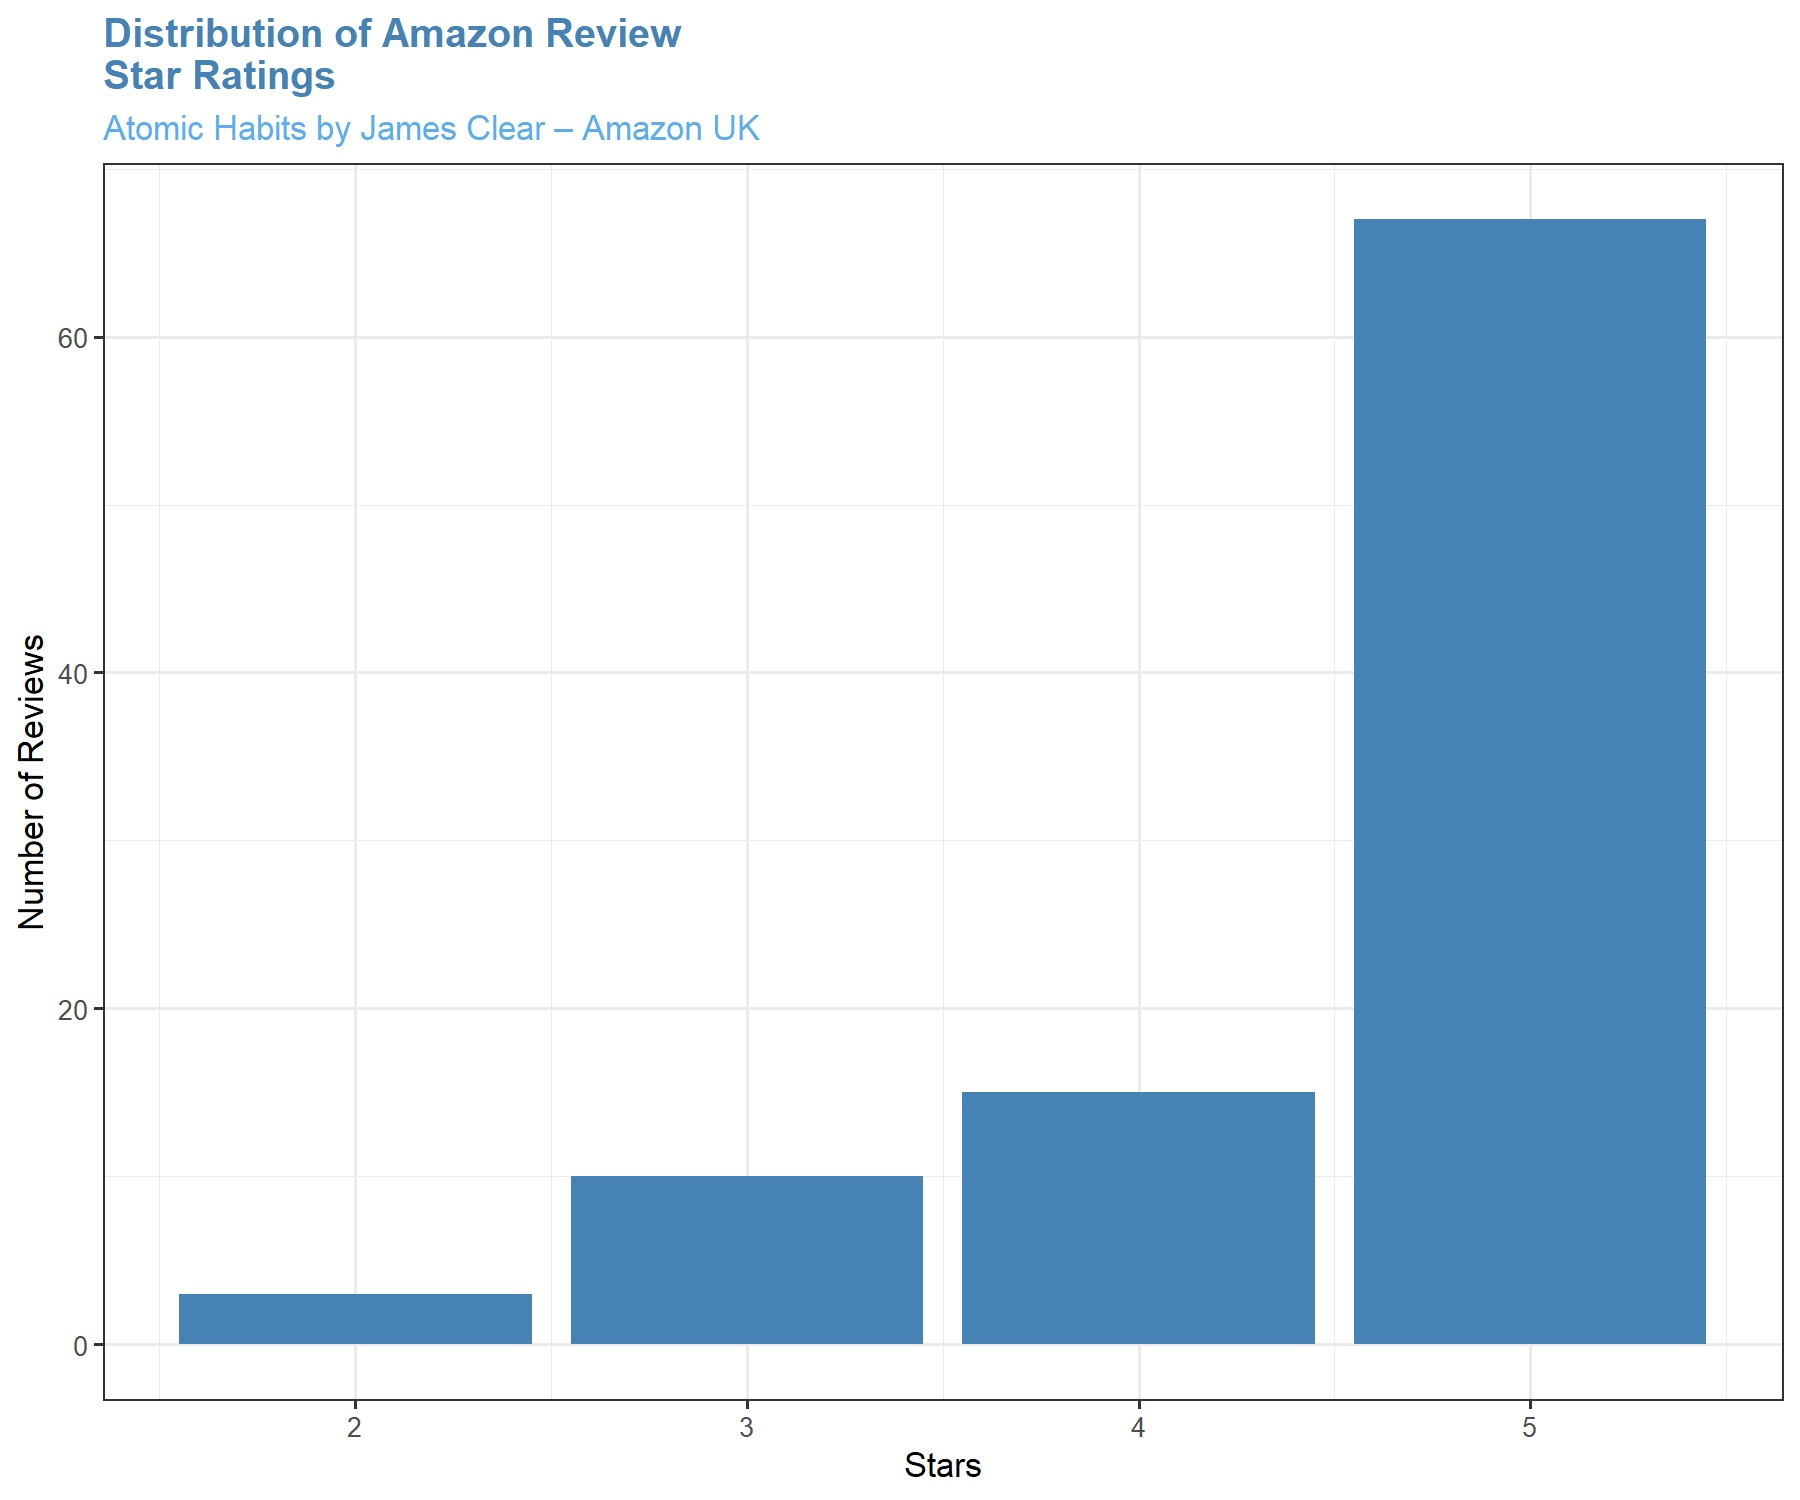
\includegraphics[width=\textwidth]{fig1a.jpeg}
\end{subfigure}
\hfill
\begin{subfigure}{0.45\textwidth}
\centering
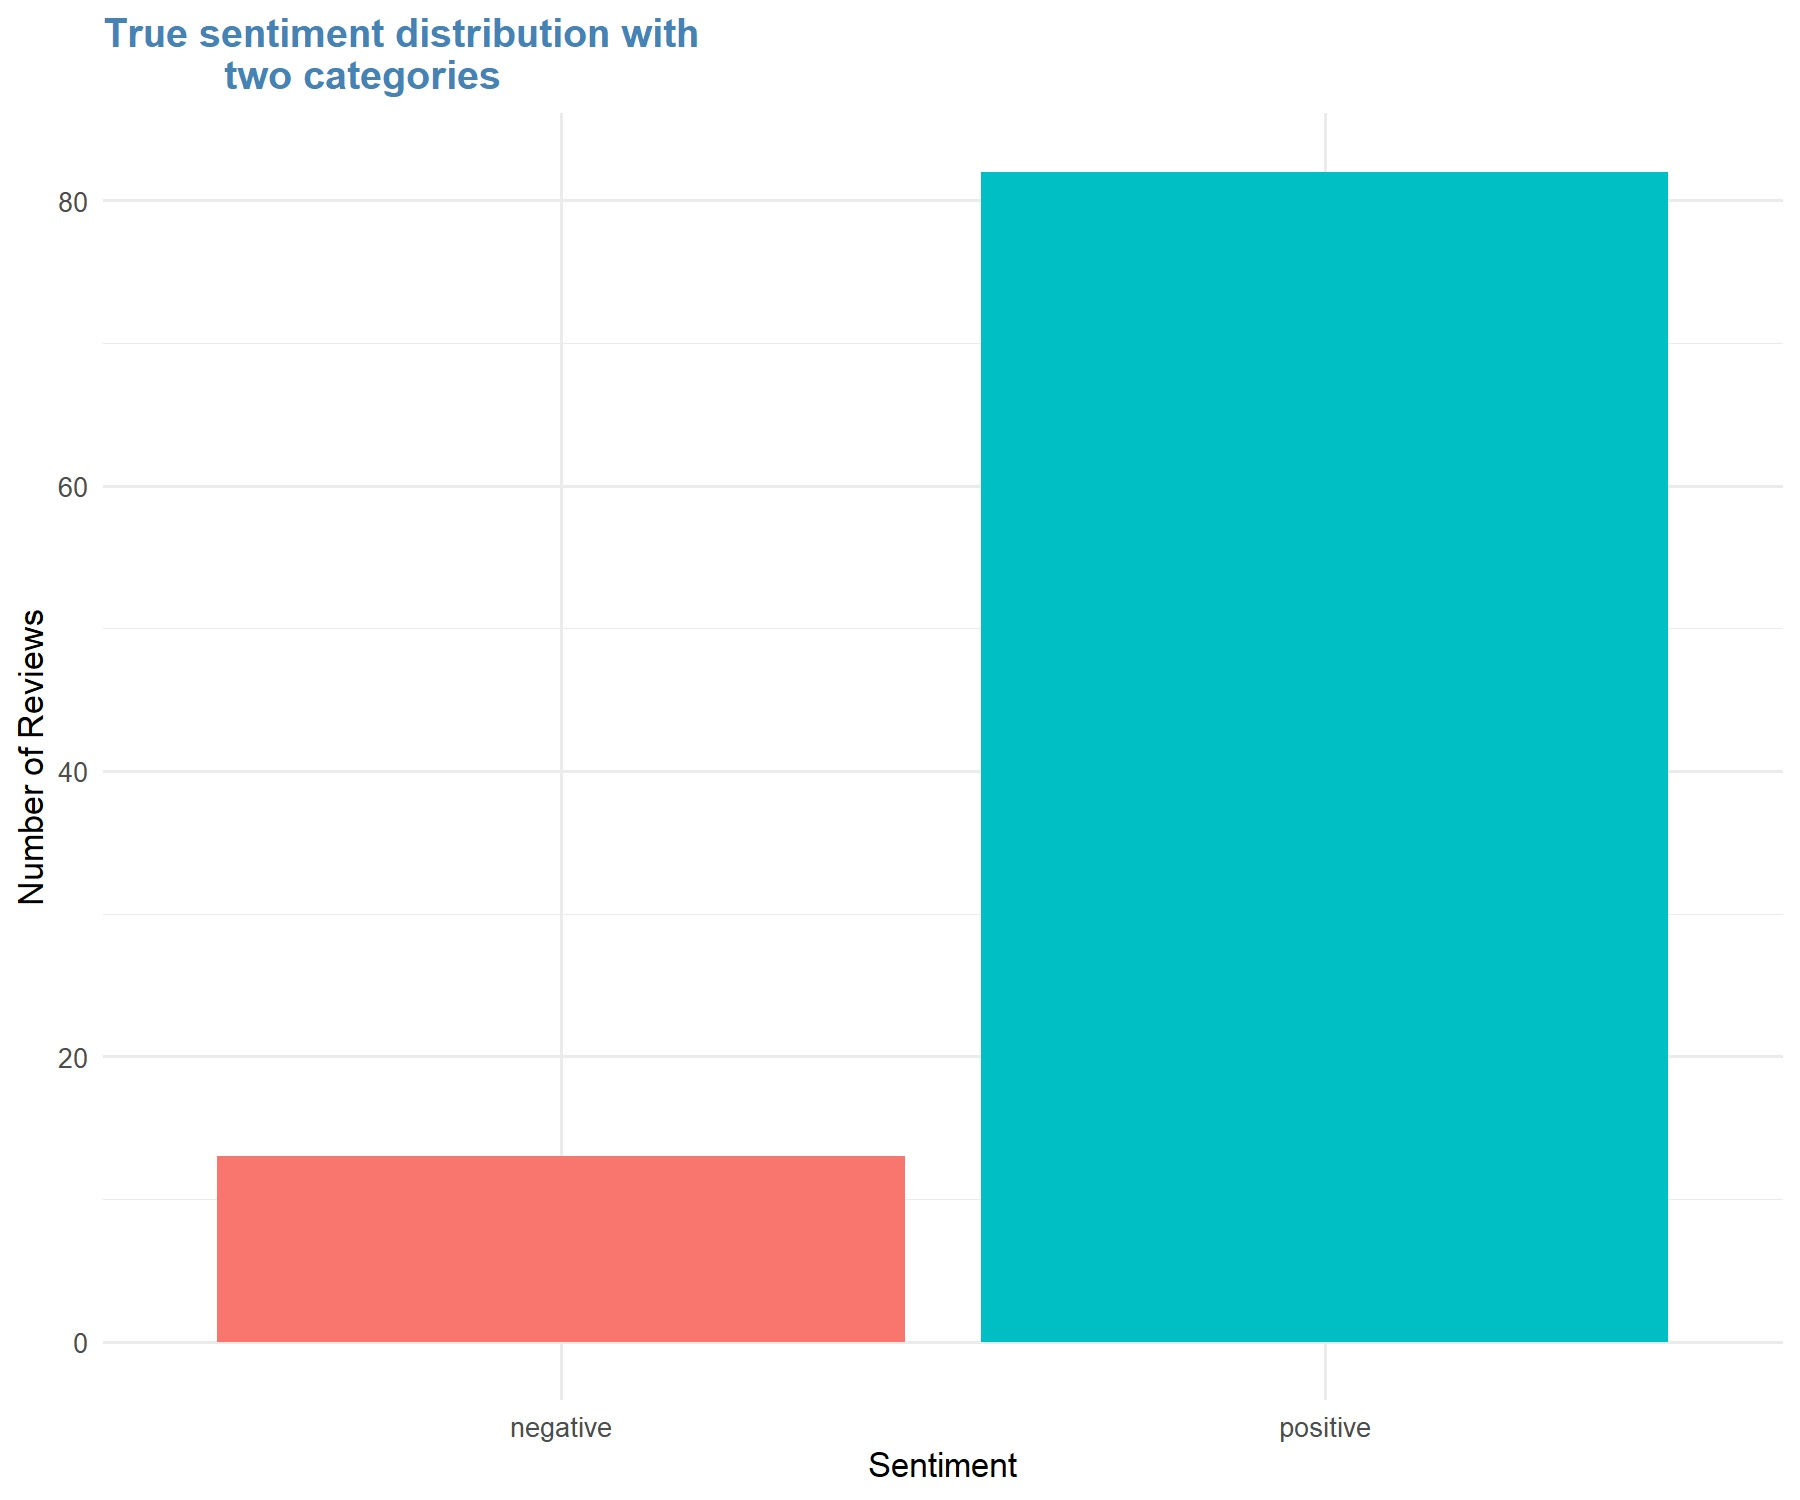
\includegraphics[width=\textwidth]{fig1b.jpeg}
\end{subfigure}
\caption{Distribution of star ratings (left) and of the binary sentiment variable \texttt{star\_sent} (right).}
\label{fig:explore}
\end{figure}

\begin{figure}[h]
\centering
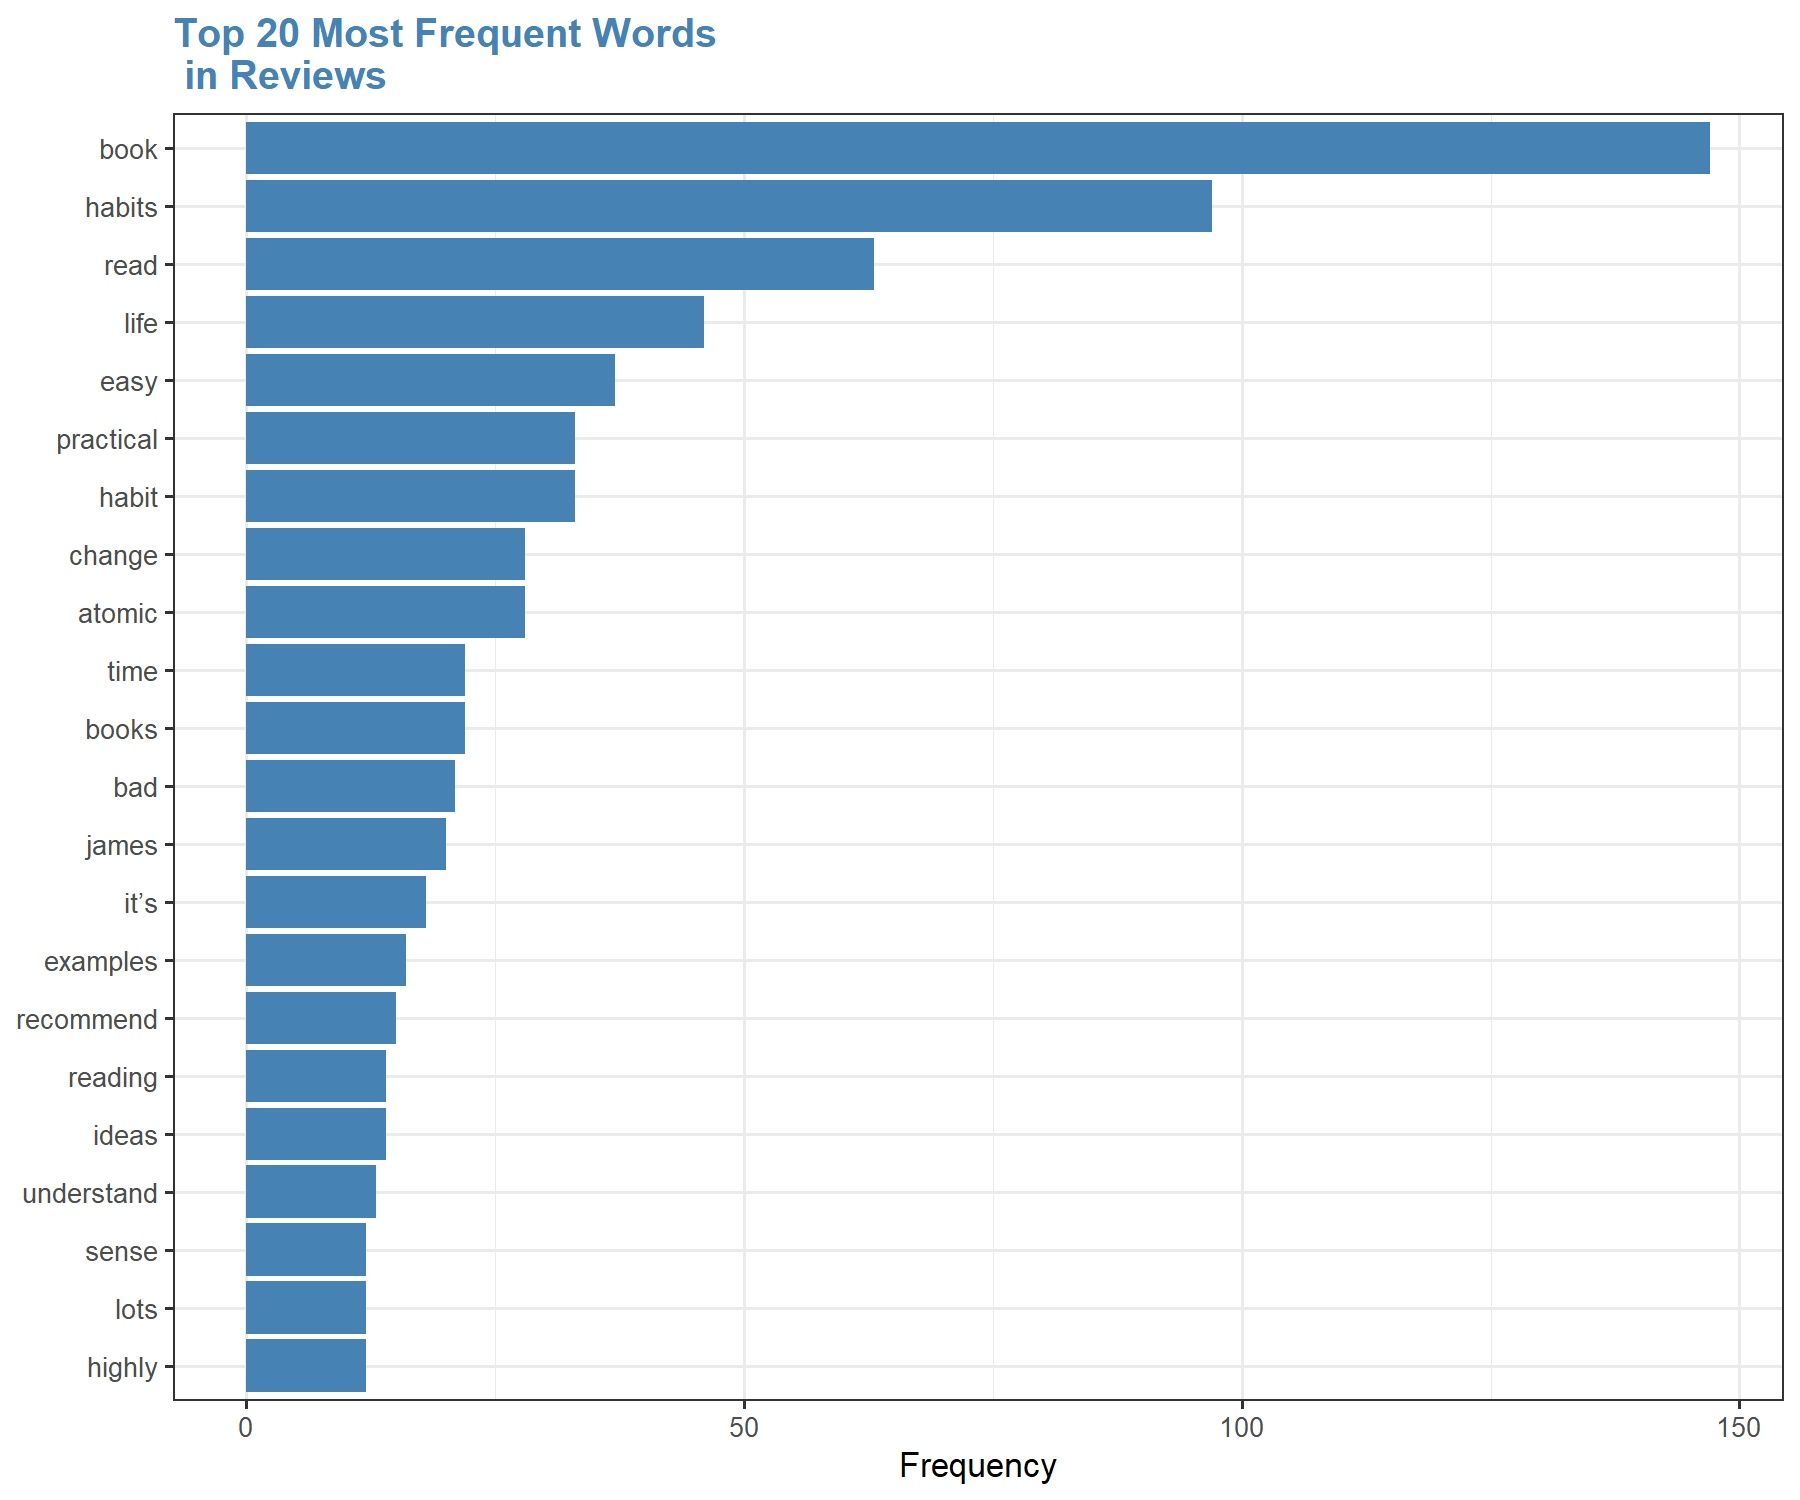
\includegraphics[width=0.55\textwidth]{fig2.jpeg}
\caption{Twenty most frequent words after stopwords removal.}
\label{fig:topwords}
\end{figure}

\subsection{Bing Lexicon}

For the Bing lexicon method, we took each review, tokenized it, and then checked those words against our list. We counted how many positive words there were and subtracted the negative ones to get a score. We did this twice: once after removing the stopwords, and once with them still in. This was to see how cleaning up the text affected things.

Removing the stopwords meant fewer reviews actually matched any words in our list, so we couldn't score as many. Keeping them meant more reviews had a score, but sometimes normal words like ``well'' or ``like'' could unfairly bump up or down the score. We decided that if a review had an equal number of positive and negative words (a score of zero), we'd count it as negative. We figured a score of zero means there is no positive signal, rather than a real sign of positivity. Then we compared scores with \texttt{star\_sent} using confusion matrices. Figure~\ref{fig:bingwords} shows which words drove the scores, with and without the stopwords removed.

\begin{figure}[h]
\centering
\begin{subfigure}{0.48\textwidth}
\centering
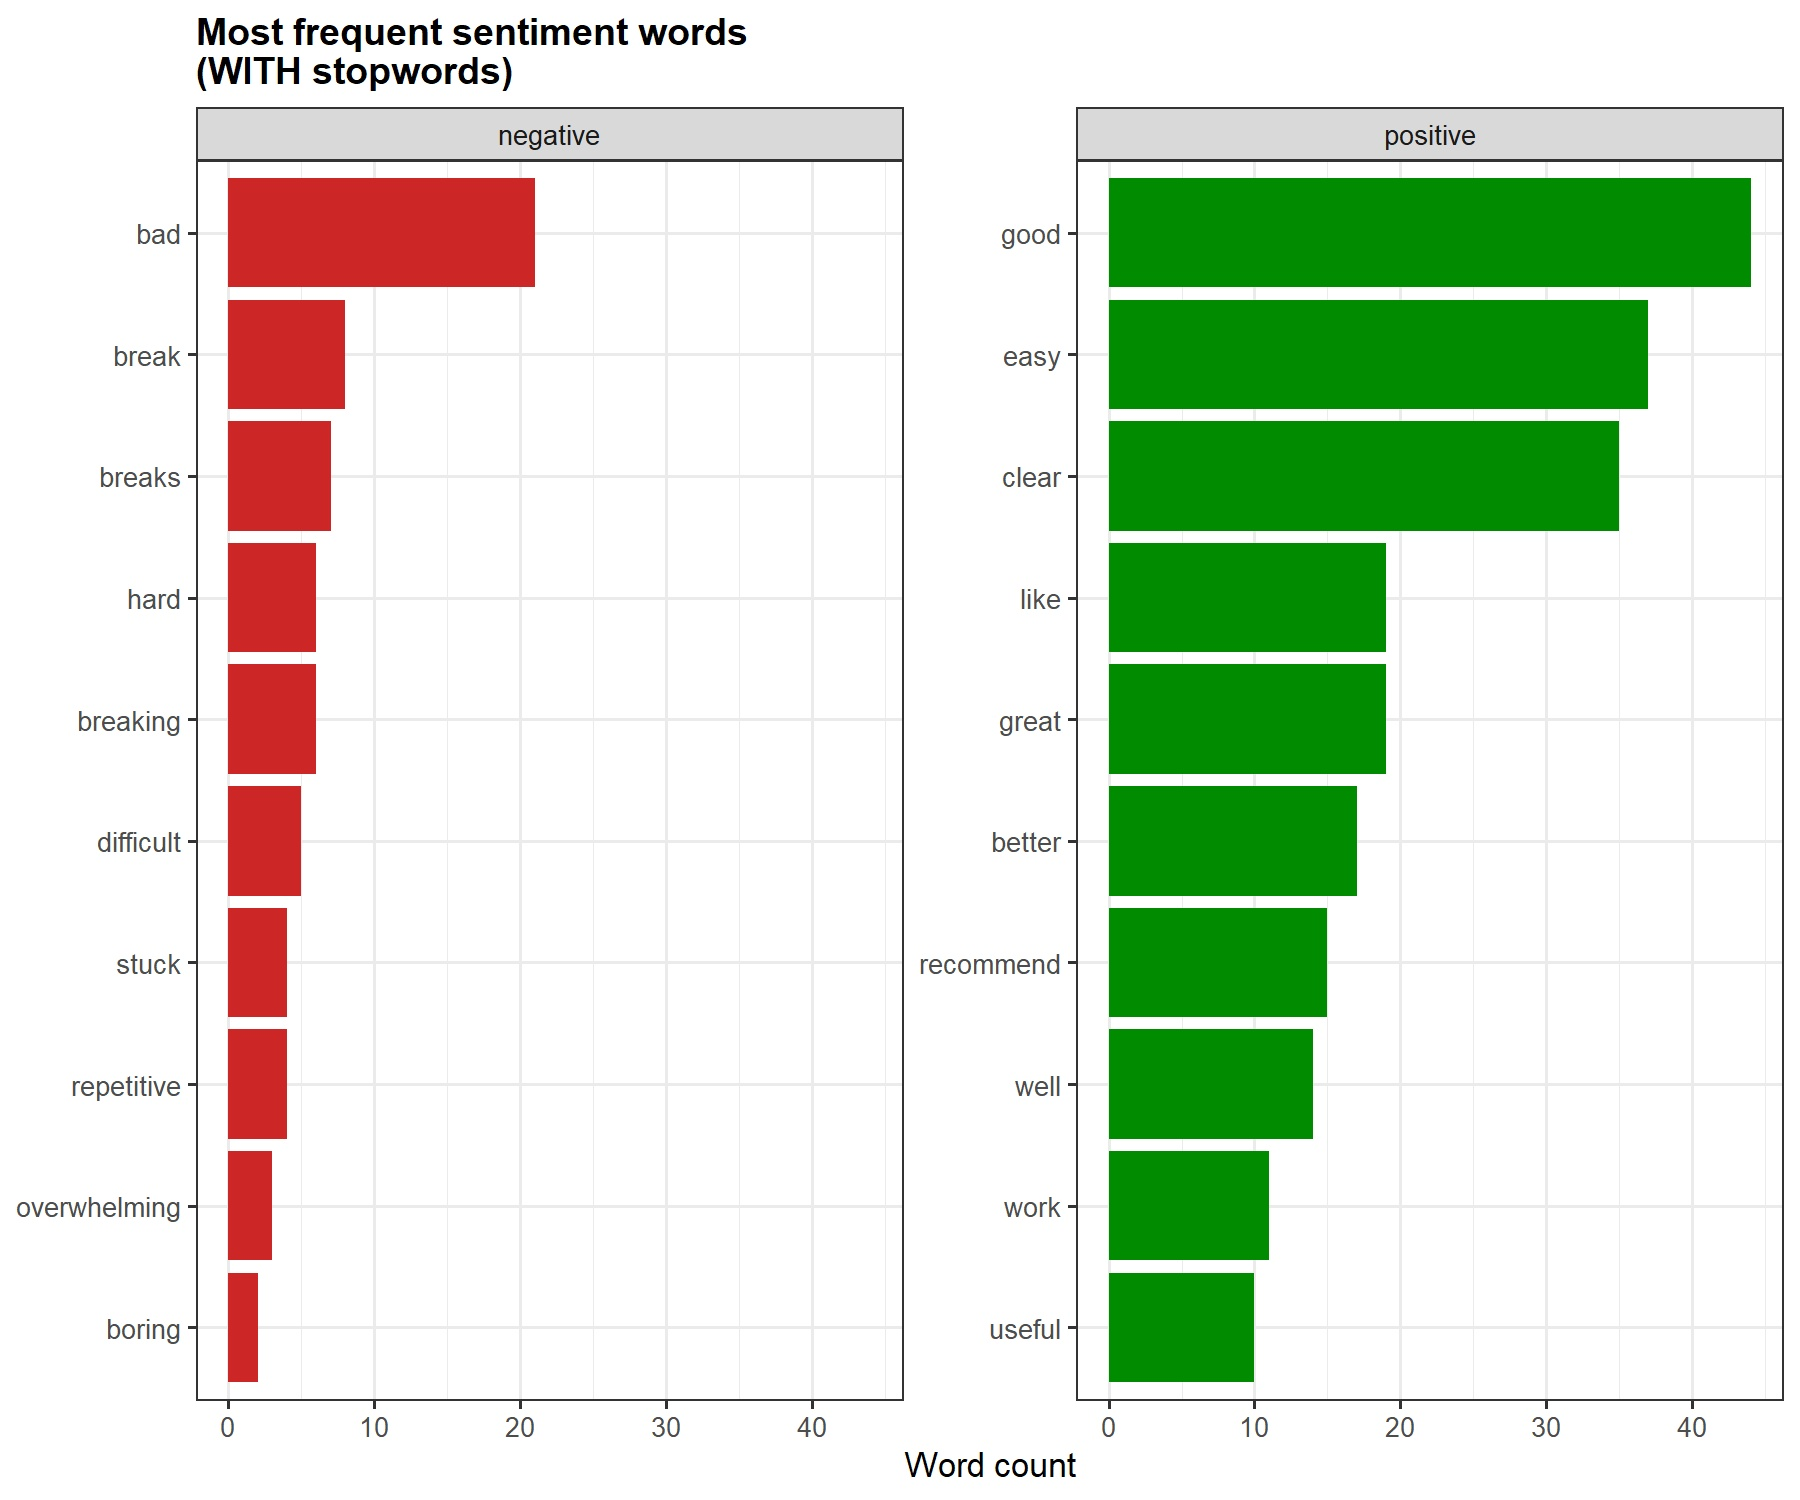
\includegraphics[width=\textwidth]{fig3a.jpeg}
\end{subfigure}
\hfill
\begin{subfigure}{0.48\textwidth}
\centering
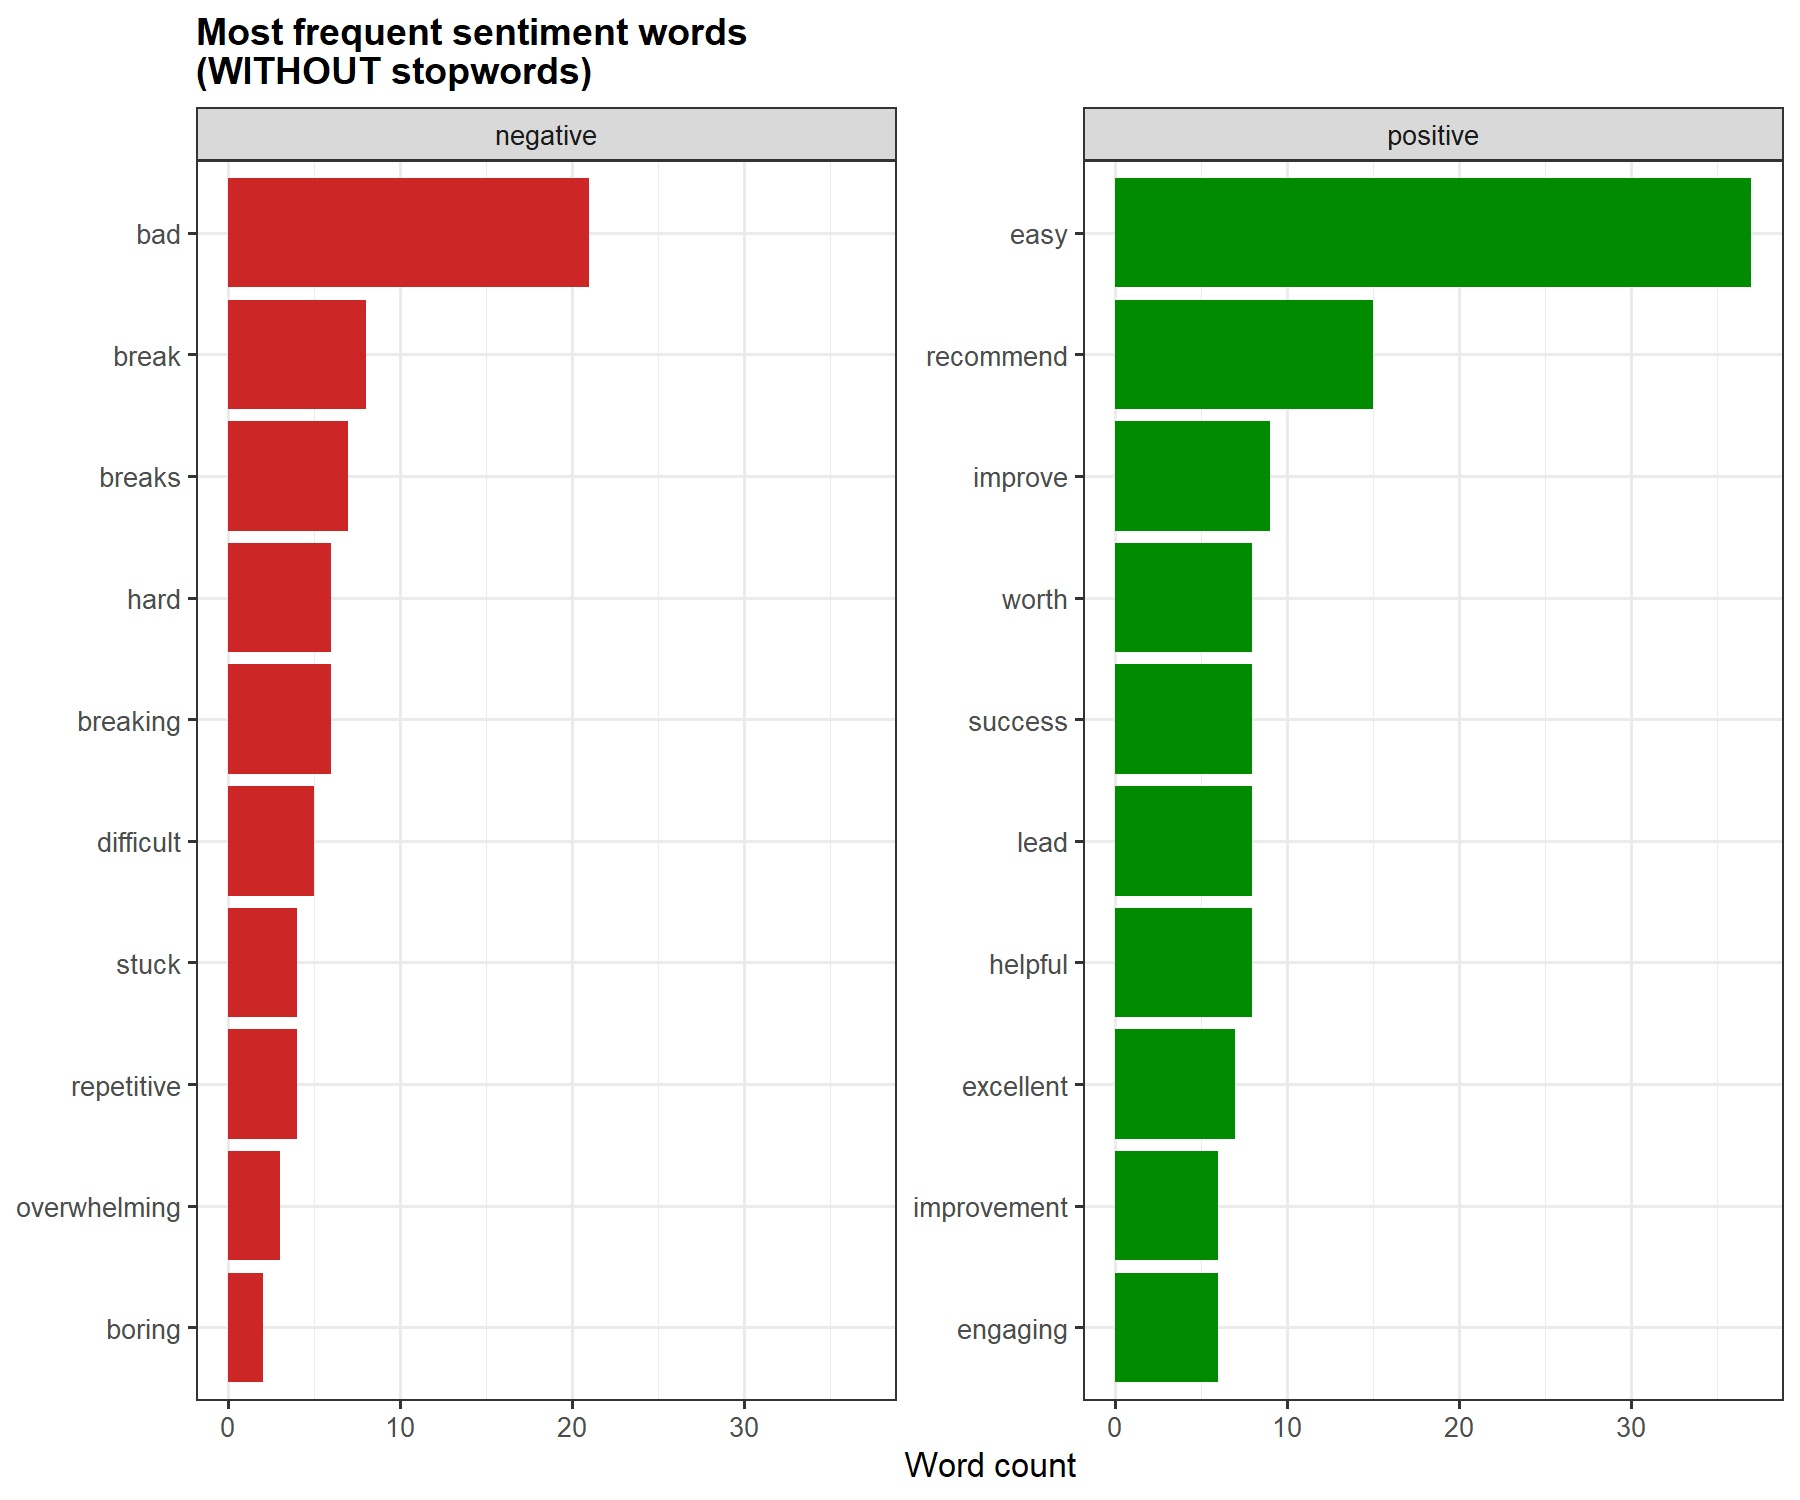
\includegraphics[width=\textwidth]{fig3b.jpeg}
\end{subfigure}
\caption{Most frequent sentiment words with stopwords (left) and without stopwords (right).}
\label{fig:bingwords}
\end{figure}

\subsection{UDPipe}

Next, we used UDPipe, a more advanced tool, on the reviews, using a specific English language model called GUM. We then reformatted our Bing lexicon so it worked with UDPipe. We tried two ways. The first, a basic version, applied the lexicon to the lemma of each word, without taking negators or amplifiers into account. The second version added in words that negate meaning (negators, like ``not'') and words that amplify or reduce the impact of other words (amplifiers and deamplifiers, like ``very'' or ``quite''). We gave the amplifiers a weight of 0.8 and looked at words within three places before and after a sentiment word. We picked the most common adverbs in the reviews as our amplifiers and deamplifiers.

\subsection{Naive Bayes}

The Naive Bayes classifier used \texttt{star\_sent} as the label. We tokenized the reviews using quanteda, got rid of punctuation, numbers, and stopwords, and then shortened the words to their basic form (stemming). This showed which words were in the reviews. We then trained the classifier on about 70 percent of the reviews (66 documents) and tested it on the remaining 29, making sure it only looked at words it had seen during training.

\subsection{Comparison of All Methods}

To compare everything fairly, we only used the 29 reviews that all the methods had access to. We then calculated how accurate each method was and compared them. The methods we tested were: Naive Bayes, Bing with stopwords, Bing without stopwords, udbing, and udpipe.

\subsection{Quantitative Results}

Out of the 95 reviews, 82 were positive and 13 were negative. So, about 86 percent of reviews were positive. Scores averaged 4.54, and the middle score was 5 stars.

When we looked at all 95 reviews, the accuracy scores were as follows.

\begin{table}[h]
\centering
\caption{Full dataset results}
\begin{tabular}{lcc}
\toprule
Method & Accuracy & Sensitivity \\
\midrule
Bing, no stopwords & 0.66 & 0.45 \\
Bing, stopwords    & 0.84 & 0.27 \\
UDbing             & 0.82 & 0.46 \\
UDpipe             & 0.82 & 0.54 \\
\bottomrule
\end{tabular}

\vspace{0.5em}
{\small No Information Rate (majority class) = 0.86.}
\end{table}

Noticed two things. All the methods were pretty good at figuring out the positive reviews, which made up most of our data, as the high specificity shows. However, they all struggled with the small number of negative reviews, which is what the sensitivity column captures: it ranges from 0.27 (Bing with stopwords) to 0.54 (UDpipe), so between roughly half and three quarters of the negative reviews were missed. Since the full dataset only had 13 negative reviews, it's hard to be super confident in these numbers, and no method clearly beat the No Information Rate of 0.86. So, the ranking is more of an indication.

On the smaller, common 29-document test set, the results were as follows.

\begin{table}[h]
\centering
\caption{Common 29-document test set results}
\begin{tabular}{lc}
\toprule
Method & Accuracy \\
\midrule
UDpipe             & 0.86 \\
UDbing             & 0.79 \\
Bing, stopwords    & 0.76 \\
Naive Bayes        & 0.72 \\
Bing, no stopwords & 0.72 \\
\bottomrule
\end{tabular}
\end{table}

\begin{figure}[h]
\centering
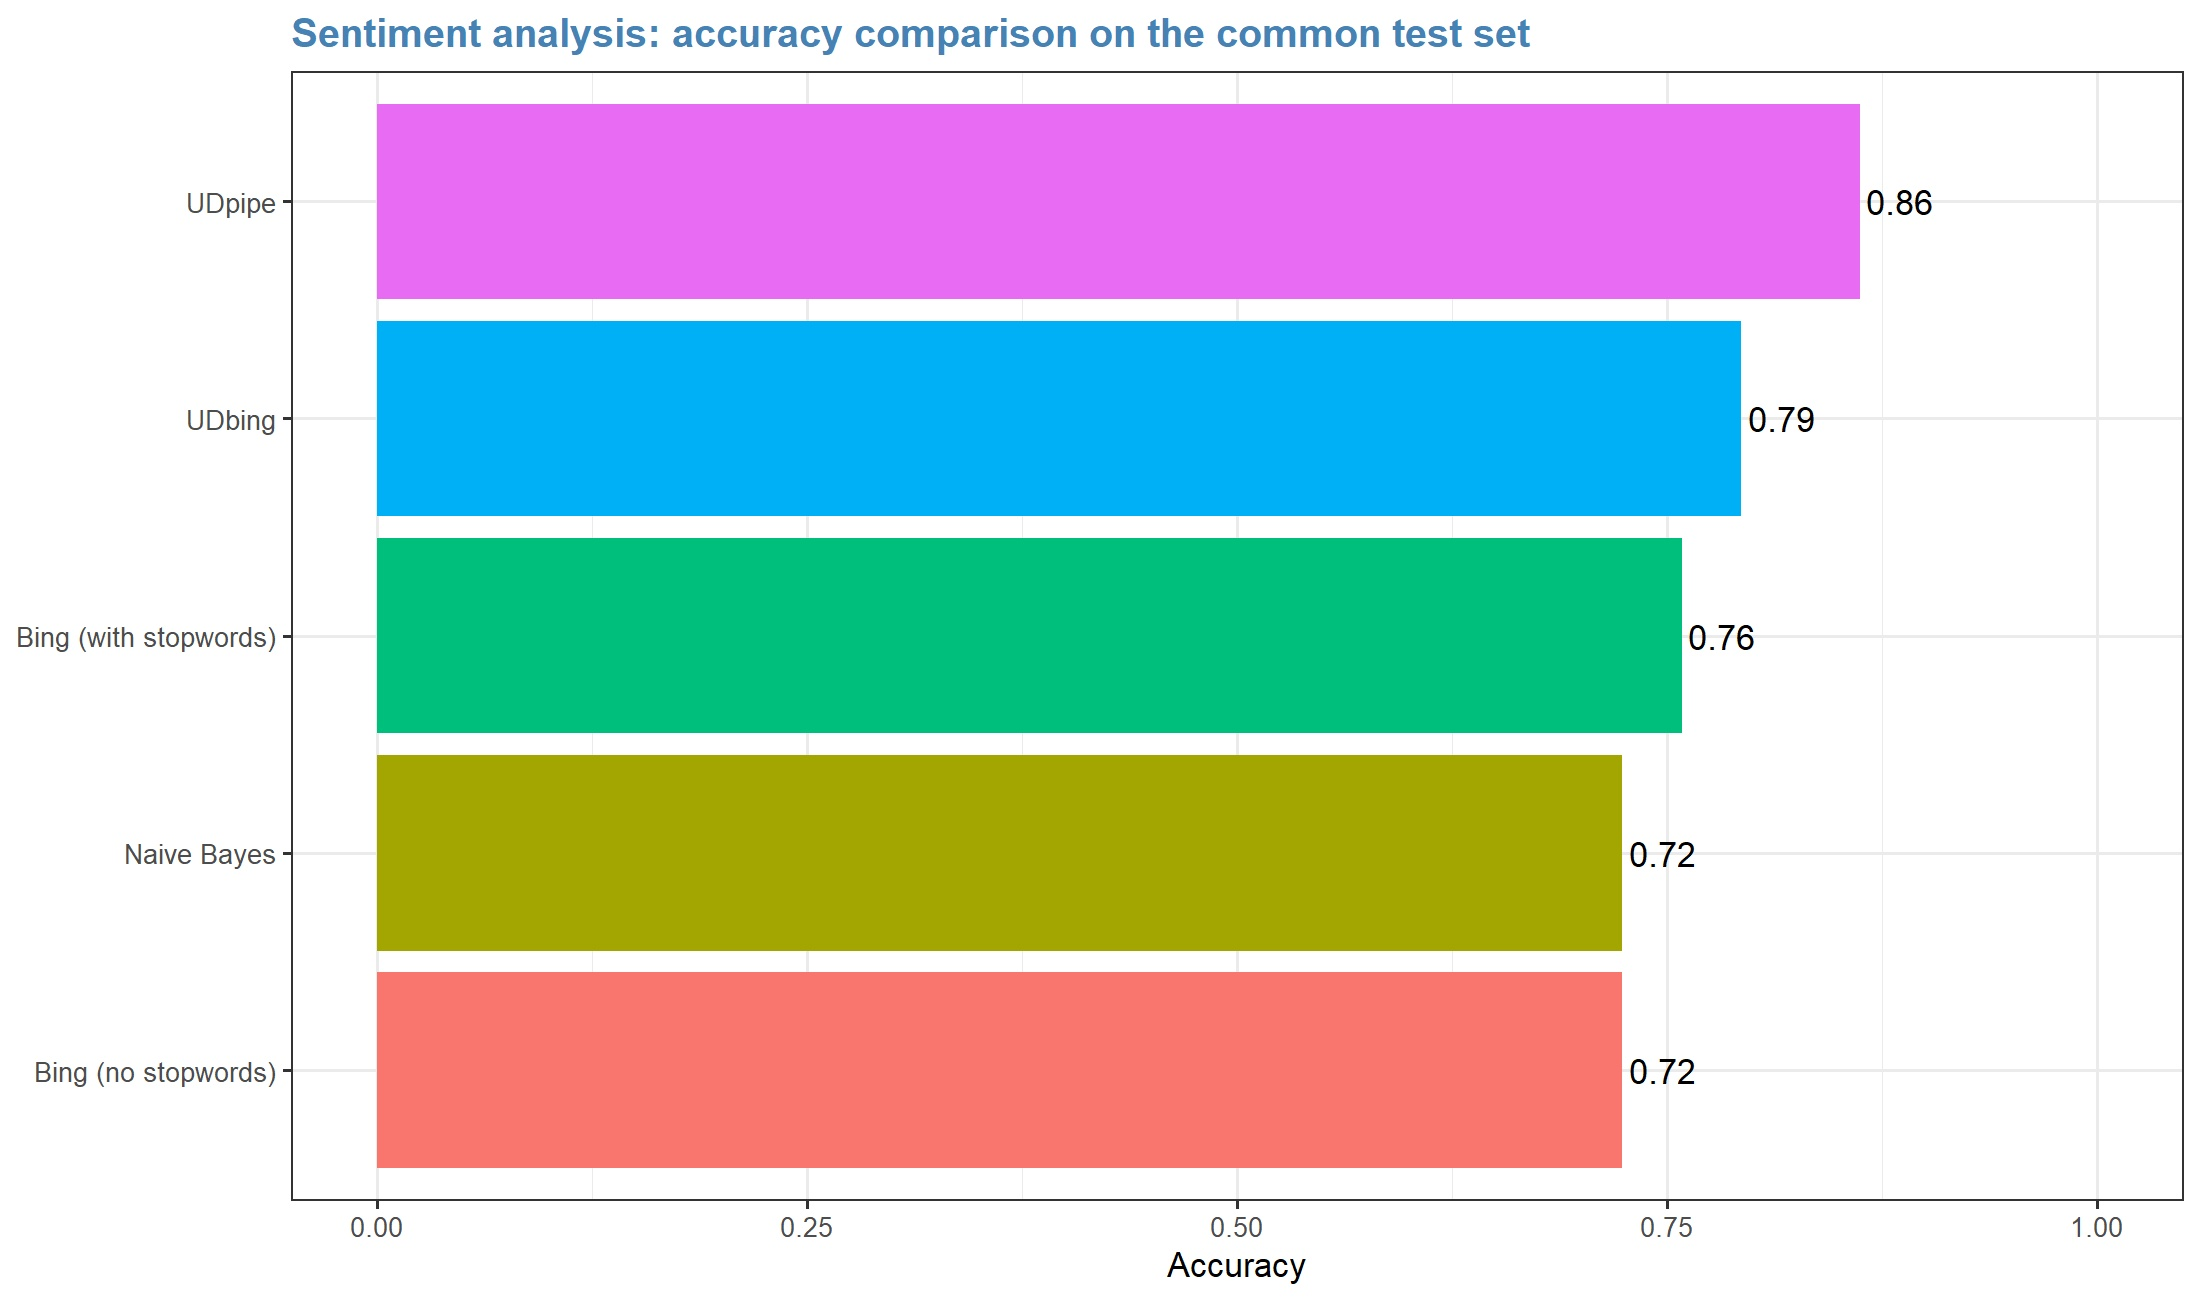
\includegraphics[width=0.7\textwidth]{fig4.jpeg}
\caption{Accuracy comparison of the five methods on the common test set.}
\label{fig:acc}
\end{figure}

\section{Conclusions}

These dictionary methods are easy, and don't need extra training. Their downsides are that they might not have all the words you're looking for in their lists and how you clean the text can really change the results. UDpipe came out as the best method: it was the most accurate on the common test set (0.86), and on the full dataset it caught more of the negative reviews than any other approach. The UDPipe modifiers (negators like ``not'' and amplifiers like ``very'') clearly helped here. Comparing UDpipe to UDbing isolates their effect, since the two share the same lexicon and model and differ only in whether the modifiers are used: adding them raised the sensitivity on negative reviews from 0.46 to 0.54, while keeping the same overall accuracy. So accounting for negation and intensity made the method better exactly where all the others struggled. Naive Bayes can learn unique words from the specific reviews it sees, but you need reviews that are already labeled with their sentiment, and you need a separate set of reviews to test it on.

The biggest problem here is the uneven number of positive and negative reviews. With so many positive reviews, any method that just defaults to calling everything positive will look more accurate than it really is. We could say more if the reviews were better and we used more ways to check accuracy. Among the methods we tried, UDpipe was the strongest, mainly because handling negation and intensity helped it on the negative reviews the others kept missing. Bing's simple, and Naive Bayes works for lots of text types, but on these reviews the modifier-aware UDpipe had the edge.

\end{document}